\documentclass[size=11pt]{report}

\usepackage{authblk}
\usepackage{fancyhdr}
\usepackage{graphicx}
\usepackage{indentfirst}
\usepackage[portuguese]{babel}

\title{TP2}
\title{
    Comunicação por Computador \\
    \large{Trabalho Prático 3}
}

\author{
    Cristiano Pereira A93726 \\
    Marco Costa A93283 \\
    Hugo Fernandes A89481
}

\affil{
    Universidade do Minho \\
    Departamento de Informática
}


\begin{document}
    \maketitle
    \newpage

    \section*{Parte I}
        \subsection*{1}
            \noindent
            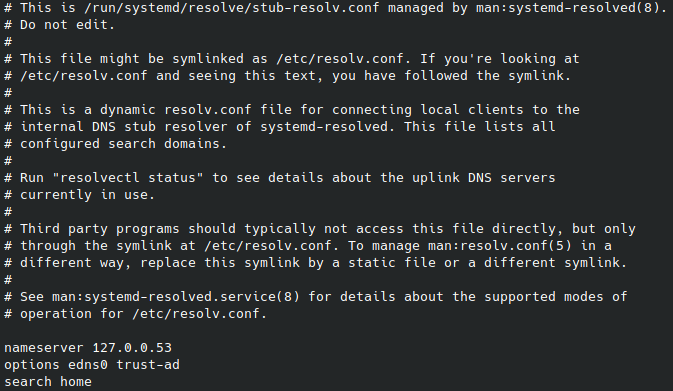
\includegraphics[width=\textwidth]{images/resolv.conf.png}
            \par
                    O ficheiro \textit{/etc/resolv.conf} é lido pelas rotinas do resolver para saber
                a que servidor de DNS se deve conectar, bem como outras informações de configuração.\par 
                    Na imagem acima pode ser visto todo o conteúdo deste ficheiro. Para além de várias linhas de comentários
                podem ser lidas três linhas que dizem ao \textit{resolver} como se comportar. Esta máquina foi configurada com os seguintes parâmetros: 
                \begin{description}
                    \item[nameserver 127.0.0.53] Diz ao \textit{resolver} a que servidor DNS se deve conectar. Neste caso aponta para o endereço 127.0.0.53 no
                    \textit{localhost} onde opera o processo \textit{systemd-resolved} que toma conta do processo de encaminhamento dos pedidos.
                    \item[options edns0 trust-ad] Permite mudar as variáveis internas do \textit{resolver}.
                    \item[search home]   
                \end{description}
            \pagebreak
        \subsection*{2}
\end{document}